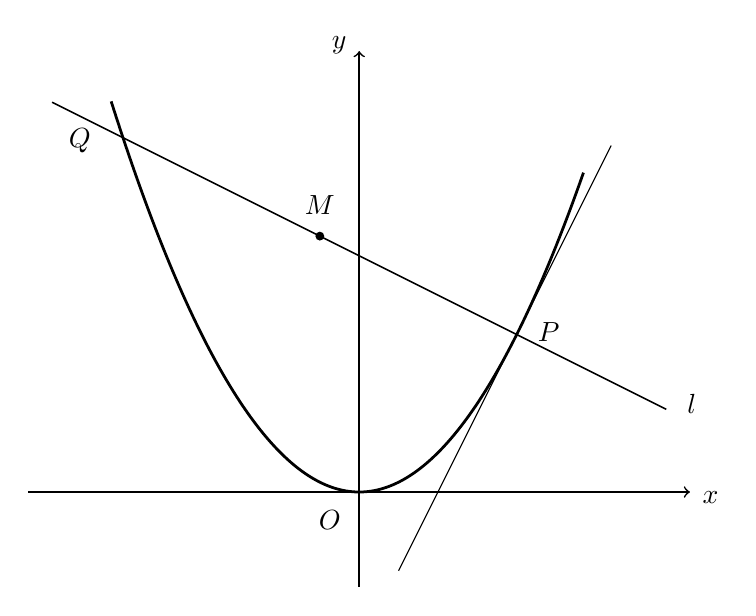
\begin{tikzpicture}[x=1cm,y=1cm,line width=0.6pt,font=\normalsize]
% axes
\draw[->] (-4.2,0)--(4.2,0) node[below=2pt,right=1pt] {$x$};
\draw[->] (0,-1.2)--(0,5.6) node[above=2pt,left=1pt] {$y$};
\node[below left=3pt] at (0,0) {$O$};
% parabola y=0.5x^2 generated from formula, domain covers Q and P
\draw[line width=1.0pt] plot[domain=-3.15:2.85,samples=140] (\x,{0.5*\x*\x});
% secant line l through P(2,2) and Q(-3,4.5): y=-0.5x+3
\draw[solid] (-3.9,4.95)--(3.9,1.05) node[right=4pt,yshift=2pt] {$l$};
% tangent at P: y=2x-2, short segment near P
\draw[solid,thin] (.5,-1)--(3.2,4.4);
% points P, Q, M (M midpoint of PQ)
\coordinate (Pp) at (2.0000000000,2.0000000000);
\coordinate (Qp) at (-3.0000000000,4.5000000000);
\coordinate (Mp) at (-0.5000000000,3.2500000000);

\fill (Mp) circle (1.6pt);
% Q lies on parabola/line intersection, marked by crossing (no dot in original)
% labels offset from strokes
\node[right=4pt,yshift=1pt] at (Pp) {$P$};
\node[left=5pt,yshift=-1pt,xshift=-3pt] at (Qp) {$Q$};
\node[above=4pt] at (Mp) {$M$};
\end{tikzpicture}
